\chapter{Simulation studies for proton computed tomography} \label{sec:setup}
With the demonstration of Corryvreckans validity as a track reconstruction framework, its performance for conditions present
in proton computed tomography scans can be investigated. The telescope used to reconstruct the protons consists of six IBL planar sensors
grouped into two triplets. Due to the fact that the spatial resolution of the sensors is five times better in the horizontal direction, the middle sensor
of each triplet is rotated by 90°. This way the lower track reconstruction precision in the vertical direction is partially compensated for.
The setup for proton computed tomography is shown schematically in figure \ref{fig:phantom} with an IBL sensor in between the triplets serving as a DUT instead of a patient. \\
For proton computed tomography it is necessary that the protons can to traverse the entire telescope including the patient
to measure their remaining energy, which is the reason the energy of the proton beam has to be significantly higher than during
the proton therapy. Current proton synchrotrons used in proton therapy centers have an upper energy limit of $200 - \SI{250}{\mega\eV}$.
Therefore, a $\SI{200}{\mega\eV}$ proton beam is used in this analysis.

\begin{figure}
  \centering
  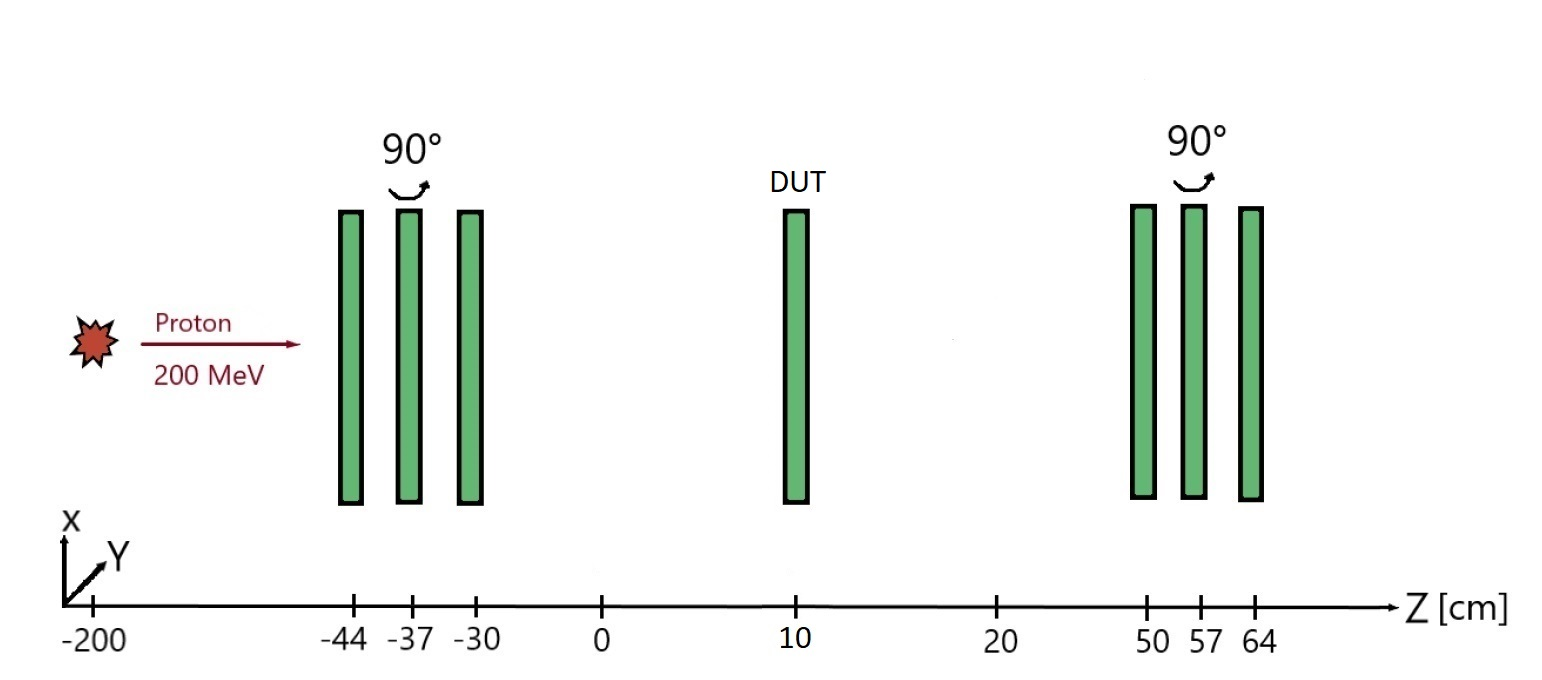
\includegraphics[height=0.45\textwidth]{images/phantom_proton_4.jpg}
  \caption{Schematic representation of the telescope used for the reconstruction of proton computed tomography. For the real
  application, a patient replaces the DUT sensor.}
  \label{fig:phantom}
\end{figure}

Since the tracking performance of Corryvreckan will be investigated, no
phantom will be present in the setup as it would
increase the number of multiple scatterings and significantly decrease the number of protons passing the telescope. Instead, another
IBL planar sensor is placed directly in the middle of the telescope serves as a DUT.

To analyse Corryvreckans performance in reconstructing proton tracks, data fed into the framework is simulated by the Allpix$^2$ software,
which is explained in the following section.

\section{The simulation software Allpix$^2$}
Allpix$^2$ is a generic simulation framework developed at CERN to simulate the performance of silicon detectors and was released in 2017.
It builds upon the
Geant4 \cite{geant4} package to perform tasks in the simulation chain. The main tasks of Allpix$^2$ are the simulation of energy depositions of particles
in the sensors, the propagation of charge carriers in the sensor material, and the digitization of the signal. It has a modular
structure to ensure easy handling, while still allowing for complex detector simulations.
Instantiation and processing of the modules are done by the core of the framework,
which contains five subsystems. This includes the configuration containing the configuration manager, which grants access to the configuration file, the
module subsystem, which loads and executes the modules, and the geometry subsystem, which provides the information of the telescope setup.
Objects are transferred from one module to another with the messenger subsystem.
Figure \ref{fig:allpix} depicts the overall structure of Allpix$^2$.

\begin{figure}
  \centering
  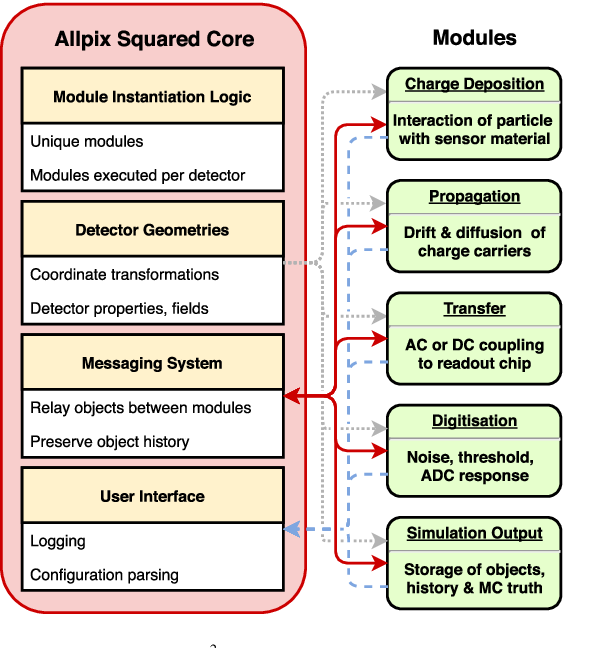
\includegraphics[height=0.5\textwidth]{images/allpix.png}
  \caption{Schematic representation of the overall Allpix$^2$ structure \cite{fig_allpix}.}
  \label{fig:allpix}
\end{figure}

The telescope geometry has to be specified in a geometry file, which includes all sensors and their pixel matrix as well as their spatial and time
resolution. Additionally,
the position and orientation have to be stated. Optionally, uncertainties on the position and orientation can be set to account for misalignment in real
telescope setups.
In the configuration file, the geometry is imported as well as the modules for the simulation in order of execution, which
will be explained in the following.

The world frame of the simulation is created with the GeometryBuilderGeant4 module. The world material can be either air or vacuum with a configurable world margin percentage.
Afterwards, all detectors from the internal detector models and passive material models are created according to the specifications in the geometry file.

Charge carriers are deposited in the active volume with the DepositionGeant4 module, which initializes the simulation of particles. The shape of the source beam, as well
as the type of particle and its energy, can be specified. Further parameters are the width of the beam, its angular distribution based on Gaussian distribution, and the energy
uncertainty of the simulated particles. All particles created at the same time define an event. The number of generated electron-hole pairs is calculated with the
mean pair creation energy and is subject to fluctuations, which are defined by the fano factor.

An electric field is added to the sensors with the ElectricFieldReader module. By default, all sensors are targeted by the module, though specific sensors can be stated.
There are three types of electric field models available, constant electric fields, linear electric fields, and external simulated electric fields, with only
linear electric fields being used in the scope of this thesis. The constant slope of linear electric fields is defined by the bias voltage and the
depletion voltage of the sensor. Optionally, the depletion depth instead of the depletion voltage can be specified.

Either with the ProjectionPropagation or the GenericPropagation module, the transport of charge carriers through the sensitive material is simulated.
The first module projects electrons or holes onto the surface and performs a randomized diffusion based on a two-dimensional Gaussian distribution around
the projection. Using an approximation of the drift time makes it possible to determine the diffusion width under the assumption of a linear electric field. This
module saves computing time at the cost of accuracy. \\
The GenericPropagation module consists of a combined simulation of diffusion and drift calculated with a Runge-Kutter-Fehlberg method.
It is compatible with any electric field model and can simulate both electrons and holes
at the same time making the module
more accurate at the cost of computing time. The integration time can be specified by the user to determine the time of the propagation process. \\
In both modules, charge carriers are combined into sets and propagated together with no interaction between them. The set size of charge carriers can be specified by the user,
making it possible to control the accuracy and computing time of the simulation. For diffusion simulations, it is necessary to specify the temperature of the sensor material
to calculate the diffusion constant.

Sets of charges are combined on the sensor pixels with the SimpleTransfer module and are prepared  to be processed by the front-end chips. The
propagated charges are mapped directly to the nearest pixel, while charge carriers that are outside the pixel grid or too far away from the implants are ignored.

Collected charges are then translated into digitised signals proportional to the input charge by the DefaultDigitizer module. Additionally, Gaussian noise contributions
from the readout electronics can be simulated and a signal threshold can be defined. The output signal is given in units of the electron charge per default, but
can also be given in bits by simulating a QDC converter. Optionally, a gain factor and gain smearing can be set.

Simulated events and the produced plots of the different modules are stored in a root file. With the ROOTObjectWriter module further information like propagated charge,
deposited charge, Monte Carlo (MC) particle information, and pixel hit information is stored in an additional ROOT file. Allpix$^2$ also enables the storing of
data in formats compatible with the EUTelescope and Corryvreckan software with the LCIOWriter module and the CorryvreckanWriter module respectively. Both modules possess parameters, which
determine what information of the Allpix$^2$ simulation is written into the ROOT files.

\section{Simulated setup}
Unlike conditions present in beam test experiments, protons in pct have a significant lower energy than the $\SI{5}{\giga\eV}$
electron beam produced by DESY II and a higher particle density, creating different and more complex particle tracks for
Corryvreckan to reconstruct. Since Corryvreckans performance in regards to these properties will be investigated, uncertainties
of the sensor position and orientation, as well as the beam energy and direction are set to zero. The simulated
beam has a Gaussian profile with a standard deviation of $\SI{3}{\milli\meter}$ and is orientated orthogonal to the sensor
surfaces. All information about the geometry of the telescope is specified in section \ref{sec:setup} with
figure \ref{fig:phantom} depicting the exact positions of the sensors and the beam source. \\ %The IBL planar sensor used as a DUT,
%instead of a phantom, is positioned at $\SI{10}{\centi\meter}$ along the z-axis. \\
A linear electric field with a bias voltage of $\SI{-100}{\volt}$ and a depletion depth of $\SI{200}{\micro\meter}$,
thus depleting the entire sensor volume, is specified. For the propagation of charge carriers, the more precise generic propagation
module is chosen with a room temperature of $\SI{293}{\kelvin}$ and 300 charges being propagated per step to limit the time consumption.\\
A Gaussian profile with a default standard deviation of $110$\, e as noise in the electronics is applied in the simulation.
Only pixels with a charge threshold of $600$\, e will trigger a hit.

Simulated data is written out with the CorryvreckanWriter module into a root file having the format to be read
in by Corryvreckan with the FileReader module.

\section{Proton reconstruction}\label{sec:proton_reconstruction}
Before the reconstruction of low energy protons is performed with Corryvreckan, it is crucial to understand how well the
track reconstruction works with protons and the employed telescope since proton beams are not used in major beam test
experiments for which Corryvreckan was designed. Because of that, a simulation containing 50000 protons
with an energy of $\SI{100}{\giga\eV}$ is created.
Particles in this energy region only have small scattering angles, effectively travelling
in straight lines.
No fluctuation in the proton energy is simulated and only one particle traverses
the telescope per event. All simulations in this chapter have a random seed of zero to make the results more comparable by preventing
statistical differences.
The residual in the x- and y-direction are shown in figure \ref{fig:100GeV}.

\begin{figure}
  \hspace{-1cm}
  %\centering
  \begin{subfigure}{0.53\textwidth}
      \centering
      \includegraphics[height=0.82\textwidth]{plots/100GeV_residualX_tel2.pdf}
  \end{subfigure}
  \begin{subfigure}{0.53\textwidth}
      %\centering
      %\hspace{0.95cm}
      \includegraphics[height=0.82\textwidth]{plots/100GeV_residualY_tel2.pdf}
  \end{subfigure}
  \caption{Residuals of the third plane in the x- and y-direction are shown on the left and right respectively.
  The IBL sensor has a five times larger pixel pitch in the x-direction. }
  \label{fig:100GeV}
\end{figure}

Especially notable is the five-peak structure of the residual in the horizontal direction, which is caused by the different
spatial resolution of subsequent planes. With the horizontal pixel pitch of the non-rotated sensors being
five times larger than the other two, the granularity increases by a ratio of the different pitches, in this case,
$\SI{250}{\micro\meter}/\SI{50}{\micro\meter} = 5$. This effect is shown schematically in figure \ref{fig:peaks}.

\begin{figure}
  \centering
  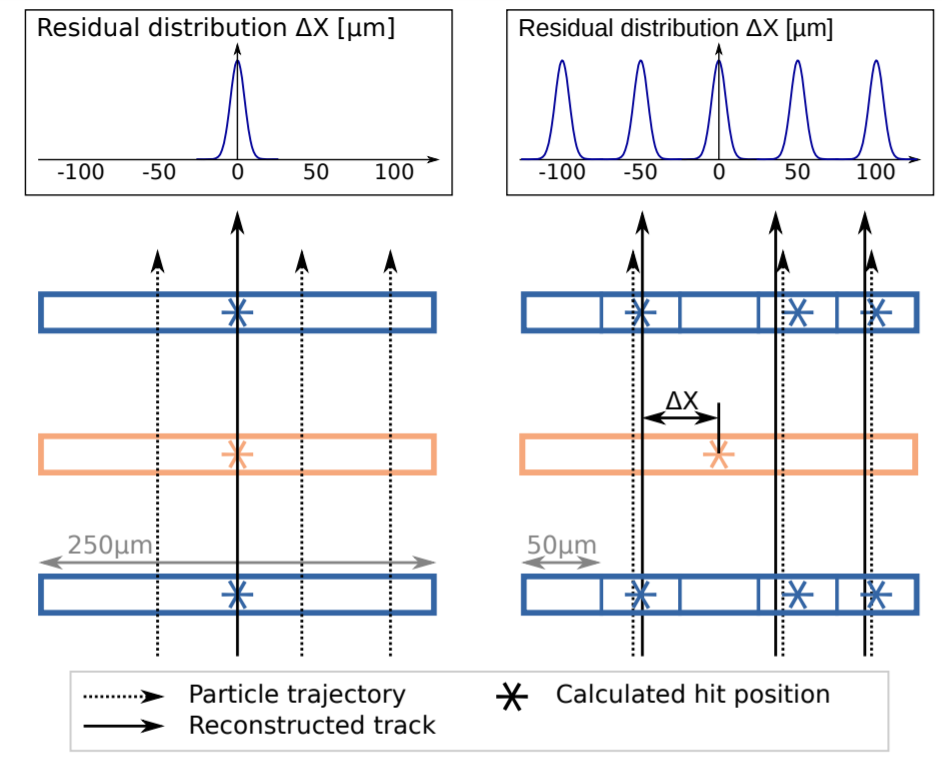
\includegraphics[height=0.6\textwidth]{images/peaks.png}
  \caption{Occurrence of a five-peak residual structure due to a different spatial resolution. The DUT in the middle
  has a five times larger pixel pitch and increases the number of peaks in its residual \cite{peaks}.}
  \label{fig:peaks}
\end{figure}

For the vertical residual of the first plane, only one peak is visible due to the lower spatial resolution, while the rotated planes
in this direction exhibit a five-peak structure. The peaks in the residual plot are narrow due to the fact that no uncertainties in regards
to the sensor positions, sensor inefficiencies, or spread in the energy of the particles are simulated. When taking these into account, the
five peaks broaden to a Gaussian profile.

The number of reconstructed tracks per event is shown in table \ref{tab:cluster_per_track} and indicates how often the proton is
reconstructed correctly. Since only one proton is simulated in an event, further reconstructed tracks arise from secondary
particles produced by the proton in an interaction. While a track fit requires a hit on all six planes, a single hit can be used by
Corryvreckan for multiple track fits, if the spatial cuts allow it. Here the spatial cuts refer to a matching radius of $\SI{750}{\micro\meter}$.
As a comparison, the track reconstruction for a matching radius of $\SI{150}{\micro\meter}$ is also listed in the table for the same
simulation.
%Any combination of clusters from the first and the last plane can
%then be connected to a track.
%Approximately $\SI{93}{\percent}$ of events were associated with a single track.

\begin{table}
  \centering
  \begin{tabular}{c | c c}
    \toprule
    Tracks per event &  $\SI{750}{\micro\meter}$ cut & $\SI{150}{\micro\meter}$ cut\\
    \midrule
    0 & 787    & 2854  \\
    1 & 48393  & 46903  \\
    2 & 643    & 104  \\
    3 & 34     & 0  \\
    4 & 3      & 0   \\
    5 & 1      & 0    \\
    6- & 0 & 0 \\
  \end{tabular}
  \caption{The number of tracks reconstructed per event for a
  $\SI{750}{\micro\meter}$ and $\SI{150}{\micro\meter}$ cut on the
  matching radius. One proton is simulated in an event, further tracks arise from clusters
  produced by secondary particles.}
  \label{tab:cluster_per_track}
\end{table}

The number of events with no reconstructed tracks increases with a smaller matching radius, as slightly non-straight paths can lead
more likely to clusters being outside of the matching radius. On the other hand, fewer tracks from secondary particles are reconstructed
for the same reason. Small cuts still lead to proper results
for reconstructing high-energy protons due to their straight path through the telescope.
%, for lower energy protons the initial $\SI{750}{\micro\meter}$ is
%used to ensure a successful association of clusters.



\section{Reconstruction of low energy protons}\label{sec:energy}
Lowering the energy of the protons in the simulation, will increase their scattering angle when interacting with the air or the sensor
planes, essentially traversing the telescope on a more complex path.
The horizontal residuals for the third plane for 50000 protons with an energy of $\SI{20}{\giga\eV}$ and $\SI{5}{\GeV}$ are shown in figure \ref{fig:20GeV}.

\begin{figure}
  \hspace{-1cm}
  %\centering
  \begin{subfigure}{0.53\textwidth}
      \centering
      \includegraphics[height=0.82\textwidth]{plots/20GeV_residualX_tel2.pdf}
  \end{subfigure}
  \begin{subfigure}{0.53\textwidth}
      %\centering
      %\hspace{0.95cm}
      \includegraphics[height=0.82\textwidth]{plots/5GeV_residualX_tel2.pdf}
  \end{subfigure}
  \caption{Residuals in the x-direction for the third plane in the telescope with a proton energy of $\SI{20}{\giga\eV}$ on the left
  and $\SI{5}{\GeV}$ on the right. A total of 50000 protons were generated in each simulation and a matching radius of $\SI{750}{\micro\meter}$ is applied. The third plane has
  a horizontal pixel pitch of $\SI{250}{\micro\meter}$.}
  \label{fig:20GeV}
\end{figure}

The five-peak structure starts to smear for $\SI{20}{\giga\eV}$ protons since the protons are more likely to scatter under larger angles causing secondary maxima.
For $\SI{5}{\GeV}$ protons, the structure is mostly vanished implying a significant number of non-linear tracks. Both simulations show that most
protons tracks can still be reconstructed.

Since the proton energy used in pct is approximately $\SI{200}{\mega\eV}$, further simulations with even lower energies are created, while all other parameters stay constant.
The horizontal residuals for proton energies below $\SI{1}{\giga\eV}$ are depicted in \ref{fig:low}.

\begin{figure}
  \hspace{-1cm}
  %\centering
  \begin{subfigure}{0.53\textwidth}
      \centering
      \includegraphics[height=0.82\textwidth]{plots/750MeV_residualX_tel2.pdf}
  \end{subfigure}
  \begin{subfigure}{0.53\textwidth}
      %\centering
      %\hspace{0.95cm}
      \includegraphics[height=0.82\textwidth]{plots/500MeV_residualX_tel2.pdf}
  \end{subfigure}
  \begin{subfigure}{0.53\textwidth}
      \hspace{-1cm}
      %\centering
      \includegraphics[height=0.82\textwidth]{plots/250MeV_residualX_tel2.pdf}
  \end{subfigure}
  \begin{subfigure}{0.53\textwidth}
      %\centering
      \hspace{-1cm}
      \includegraphics[height=0.82\textwidth]{plots/150MeV_residualX_tel2.pdf}
  \end{subfigure}
  \caption{Residuals in the x-direction for the third plane in the telescope with a proton energy of $\SI{750}{\mega\eV}$ on the upper left, $\SI{500}{\mega\eV}$ on the
  upper right, $\SI{250}{\mega\eV}$ on the lower left,
  and $\SI{150}{\mega\eV}$ on the right. A total of 50000 protons were generated in each simulation and a matching radius of $\SI{750}{\micro\meter}$ is applied. The third plane has
  a horizontal pixel pitch of $\SI{250}{\micro\meter}$.}
  \label{fig:low}
\end{figure}

All four residual plots have a defined maximum due to highly non-linear tracks. By gradually lowering the energy the standard deviation of the residual shrinks. While
it seems like the accuracy of the telescope and the track reconstruction increased, it is simply the consequence of the increasing number of protons scattering
out of the telescope, which therefore do not deposit energy in each sensor. Since this is a requirement for a reconstructed track, the number of fitted tracks decreases
noticeably, especially between $\SI{250}{\mega\eV}$ and $\SI{150}{\mega\eV}$. The first tracks that are lost for lower energies
are the ones with a high absolute value of the residual, as they are more likely to leave the telescope before traversing all sensors. \\
While the reconstruction of low energy protons and their complex path is possible, the number of reconstructable tracks decreases with lower energies.
Since it is still necessary to have a sufficient amount of tracks for a pct image, one method to counter this problem is in irradiating the patient longer.
An additional problem arises due to the increasing number of multiple Coulomb scattering inside the patient, which inevitably decreases the spatial resolution of the image.
However, the used energy reason still allows for a successful track reconstruction of protons for pct.


\chapter{Reconstruction of high track density proton beams}\label{sec:density}
Unlike in the DESY test beam facility, proton beams in proton ct tend to have a significantly higher number of particles in a sensor
per time frame. To analyse how Corrvreckan reconstructs a high track density beam, the number of particles per event in the Allpix$^2$
simulation is increased, while the proton energy is kept constant at $\SI{200}{\mega\eV}$. Other parameters are identical to previous simulations.

\section{Track multiplicities}
The track multiplicity, meaning the number of reconstructed tracks per event, for 25 and 50 particles simulated in an event is shown in figure \ref{fig:multiplicity}. To take the different spatial resolutions of the sensors in the x- and y-direction into account, a relative
spatial cut of 15.1 is applied in the reconstruction. Unlike absolute spatial cuts, relative cuts are used to define a
matching radius by multiplying the spatial resolution
of each sensor by the specified factor, creating an ellipse in the process.

\begin{figure}
  \hspace{-1cm}
  %\centering
  \begin{subfigure}{0.53\textwidth}
      \centering
      \includegraphics[height=0.82\textwidth]{plots/track_multiplicity_200MeV_25.pdf}
  \end{subfigure}
  \begin{subfigure}{0.53\textwidth}
      %\centering
      %\hspace{0.95cm}
      \includegraphics[height=0.82\textwidth]{plots/track_multiplicity_200MeV_50.pdf}
  \end{subfigure}
  \caption{Number of reconstructed tracks of $\SI{200}{\mega\eV}$ protons for 25 protons per event shown on the left and
  50 protons per event shown on the right. A total number of 50000 protons were generated in each simulation. }
  \label{fig:multiplicity}
\end{figure}

Even though the same number of protons were generated in each simulation, the mean number of tracks $\mu_{\text{Tracks}}$ reconstructed in an event
for 50 protons per event is noticeably higher, even when taking the different number of events into account. Statistically
$\mu_{\text{Tracks}}/ N_{\text{event}} \approx 0.6$ tracks per proton are created for a simulation with 25 protons per event and $\approx 1.4$ for
the 50 protons per event. In this energy region, clusters of secondary particles are negligibly rare. The cause of the
higher number of tracks in the second simulation lies in the combinatorics of fitted tracks, briefly mentioned in \ref{sec:proton_reconstruction}.
Since the reconstruction software does not know which clusters belong to a specific track, a track
is fitted through each combination of clusters from the first and the last plane within allowed spatial and time cuts.
With increasing track density, the number
of clusters within a time frame grows along with the number of possible track fits.
This also explains the far higher number of reconstructed tracks than protons simulated in certain events. \\
Additional tracks due to a higher number of clusters are problematic, as reconstructed tracks through a false
combination of clusters will cause larger errors in a proton ct image. To minimise the number of falsely reconstructed tracks
several approaches are investigated, which are addressed in the following sections.

\section{Spatial cuts for high track densities} \label{sec:cuts}
While the time resolution of the sensors in the telescope can actively contribute to lower the number of clusters within a time frame,
Allpix$^2$ automatically groups each proton simulated in an event into a single time frame, which means that no time cut will be able
to distinguish protons of the same event. However, the number of false combinatorics can be reduced by decreasing the matching radius, as
it will lower the probability of false combinations of clusters being inside the matching radius. \\
In order to be able to compare the results of different spatial cuts, it is necessary to find out how many correct and false combinations of clusters
are reconstructed. Particles simulated with Allpix$^2$ can be precisely tracked with their Monte Carlo (MC) truth information. Each exact
position of the protons on all planes can be accessed. To find correct reconstructed tracks, the MC tracks of Allpix$^2$ can be
compared with the coordinates of the cluster centers belonging to a track created by Corryvreckan. \\

The number of correct reconstructed tracks for the relative spatial cuts of 15.1 and 12.2 are given in table
\ref{tab:true_tracks} for 50000 generated protons with 10,
25, and 50 protons simulated per event.


\begin{table}
  \centering
  %\hspace{-1.5cm}
  \begin{tabular}{c | c c c}
    \toprule
     & 10 protons & 25 protons & 50 protons \\
    \midrule
    reconstructed tracks (15.1) cut & 11595 & 27726 & 68712  \\
    true reconstructed tracks (15.1) & 4709 & 4772  & 5187 \\
    ratio & 0.406 & 0.172 & 0.075 \\
    \midrule
    reconstructed tracks (12.2) cut & 5401 & 11891 & 28141 \\
    true reconstructed tracks (12.2) &  2421 &2513  & 2686 \\
    ratio & 0.448 & 0.211 & 0.095
  \end{tabular}
  \caption{Reconstructed tracks for two different spatial cuts for 10, 25 and 50 protons per event. The ratio refers to the true
  number of reconstructed tracks divided by the total number of tracks.}
  \label{tab:true_tracks}
\end{table}

With a stronger spatial cut,  the ratio of true reconstructed tracks to
the total number of tracks increases by $10.3\%$, $22.7\%$, and $26.7\%$ for 10, 25, and 50 protons per event respectively.
While this shows that stronger cuts help reducing false combinatorics, they cannot be chosen too strictly,
as the number of true tracks decreases significantly due to their high scattering angles. Even with the stricter relative cut of 12.2, the
number of true reconstructed tracks is less than half for 10 protons per event and only a 1/5 for 25 protons per event and 1/10 for 50 protons per event highlighting
the combinatorics problem. No spatial cut can achieve a ratio useful for pct, while still keeping the number
of tracks high enough for the pct to be feasible. Further approaches are therefore necessary, which are investigated in the following sections.

\section{Beam divergence for high track densities}
Another approach in limiting false combinatorics is in simulating a beam divergence to differentiate between tracks. Former simulations had no variation
in the direction of the initial protons, but an opening angle in form of a gauss profile can be specified in the DepositionGeant4 module. The specified value of
the beam divergence parameter describes the standard deviation of the Gaussian distribution of the opening angle.  \\
Three simulations of 50000 protons with 10 protons per event and three different opening angles are created.
The number of true reconstructed tracks and the ratio
of true reconstructed tracks to the total number of tracks is specified in table \ref{tab:angle}. In section \ref{sec:cuts} the method of identifying
true and false tracks in Allpix$^2$ is specified.

\begin{table}
  \centering
  \begin{tabular}{c | c c c}
    \toprule
     &  $\SI{0}{\milli\radian}$ & $\SI{2}{\milli\radian}$ & $\SI{3}{\milli\radian}$\\
    \midrule
    reconstructed tracks & 11595 & 6431 & 3948  \\
    true reconstructed tracks & 4709 & 3162 & 2267 \\
    ratio & 0.406 & 0.492 & 0.574
  \end{tabular}
  \caption{Reconstructed tracks of 50000 protons with 10 protons per event for different opening angles. The first simulation has no opening angle and the initial protons
  trajectory is perpendicular to the sensor surface. For the other simulations, the opening angle refers to the standard deviation of the Gaussian distribution of
  the opening angle. The ratio describes the number of true reconstructed tracks to the total number of reconstructed tracks.}
  \label{tab:angle}
\end{table}

The ratio of true tracks to the overall number of tracks increases with a higher standard deviation of the opening angle by $21.2\%$ and $41.4\%$ in respect to
no opening angle. Similarl to the spatial cut approach the
number of true reconstructed tracks also decreases considerably. This is due to a higher probability of particles with a large opening angle being scattered out of the telescope.
Again, tracks are only fitted, whenever a cluster is found on each of the six sensors, making this case unlikelier for wider opening angle distributions.
Even larger opening angles decrease the number of reconstructed tracks in this telescope significantly, while also being impractical for precisely irradiating a target volume.
Thus, further investigation of countering the problem of high track density beams remains necessary.

%\section{Advanced track finding algorithm for high track densities}

\section{Feature cuts for high track densities}\label{sec:feature}
Tracks inherit numerous features, which characterise them,
including their deposited energy, the kink angles, their corresponding cluster position on the sensor and the $\chi^2$ value of the track.
These features might be characteristic, meaning they differ for tracks from true and false combinations of clusters.
Analysing these properties can therefore help in differentiating true and false tracks. \\
The track features determined by Corryvreckan can be written out with the FileWriter module for further investigation.
In order to differentiate between the features of true and false tracks, the Monte Carlo truth information of the particles is used again.
A simulation containing 100000 generated $\SI{200}{\mega\eV}$ protons with 10 protons per event is created. No beam divergence and a relative spatial cut of 15.1 are applied.
Corryvreckan reconstructed a total of 23304 tracks, of which 9096 tracks have a correct combination of clusters.

Kinks describe angles, which arise due to the scattering of particles and the resulting change of direction. Particles have kinks for each sensor, with the kink being
the angle between the initial direction and the direction after scattering. These angles are crucial features of a track fit and therefore important parameters to investigate.
Figure \ref{fig:kinks} depicts the kink angles $\phi$ in the x- and y-direction for the third and fourth sensor divided in the distribution of true and false reconstructed tracks.

\begin{figure}
  %\centering
  \hspace{-1cm}
  \begin{subfigure}{0.53\textwidth}
      %\centering
      \includegraphics[height=0.82\textwidth]{plots/kink_x_3_true_false.pdf}
  \end{subfigure}
  \begin{subfigure}{0.53\textwidth}
      %\centering
      %\hspace{0.95cm}
      \includegraphics[height=0.82\textwidth]{plots/kink_y_3_true_false.pdf}
  \end{subfigure}
  \begin{subfigure}{0.53\textwidth}
    \hspace{-1cm}
      %\centering
      \includegraphics[height=0.82\textwidth]{plots/kink_x_4_true_false.pdf}
  \end{subfigure}
  \begin{subfigure}{0.53\textwidth}
    \hspace{-1cm}
      %\centering
      %\hspace{0.95cm}
      \includegraphics[height=0.82\textwidth]{plots/kink_y_4_true_false.pdf}
  \end{subfigure}
  \caption{Kink angles for the third plane in the upper row and the fourth in the lower row. The first column contains the kinks in the horizontal direction and the second column in
  the vertical direction.}
  \label{fig:kinks}
\end{figure}

All distributions follow the expected Gaussian profile around 0°, with the horizontal kink distribution being broader due to the higher pixel pitch.
While the kink distribution of true and false tracks in the vertical direction does not enable a useful
cut for track identification, the horizontal kinks of false tracks show a broader distribution in comparison to the true tracks. Therefore it is
possible to cut on the horizontal kink to reject false tracks without losing a significant amount of true tracks.
The kinks of the first and last plane can not be defined correctly and are neglected in this analysis. For the planes in the middle of the triplets, both
distributions do not enable a useful cut on the kink angle.

Another feature to investigate is the position of the cluster centers $r$ which are fitted to true and false tracks. Figure \ref{fig:clus_pos} shows the
horizontal and vertical cluster positions for true and false tracks on the last plane exemplary.

\begin{figure}
  \hspace{-1cm}
  %\centering
  \begin{subfigure}{0.53\textwidth}
      \centering
      \includegraphics[height=0.82\textwidth]{plots/global_x_6_true_false.pdf}
  \end{subfigure}
  \begin{subfigure}{0.53\textwidth}
      %\centering
      %\hspace{0.95cm}
      \includegraphics[height=0.82\textwidth]{plots/global_y_6_true_false.pdf}
  \end{subfigure}
  \caption{Distributions of the true and false tracks for the horizontal cluster position on the left and the vertical cluster position on the right.}
  \label{fig:clus_pos}
\end{figure}

While both of the distributions of the cluster positions show a greater number of false tracks in the middle of the sensor in comparison to the number of true tracks,
any cut would result in a noticeable loss of true tracks. Similar distributions of the cluster centers can be found on the other planes, which means that this feature
is not suitable for the identification of true tracks through cuts.

The last two major track features stored by Corryvreckan are the number of deposited charges of particles in each sensor and the $\chi^2$ value of the track,
which is defined in equation \ref{eqn:chi}.
Both features are shown in figure \ref{fig:charge_chi} with the charge deposition referring to the last plane exemplary.

\begin{figure}
  \hspace{-1cm}
  %\centering
  \begin{subfigure}{0.53\textwidth}
      \centering
      \includegraphics[height=0.82\textwidth]{plots/charge_6_true_false.pdf}
  \end{subfigure}
  \begin{subfigure}{0.53\textwidth}
      %\centering
      %\hspace{0.95cm}
      \includegraphics[height=0.82\textwidth]{plots/chi2_10_200MeV_xgb_true_false.pdf}
  \end{subfigure}
  \caption{Deposited charges for the last sensor on the left and the $\chi^2$ value on the right for true and false particle tracks.}
  \label{fig:charge_chi}
\end{figure}

Similar to the distribution of the cluster centers, no cut on the charge deposition is suitable to effectively sort out false tracks without losing a significant
amount of true tracks. This is the case for the charge deposition of all sensors.
The $\chi^2$ values of true and false tracks show a noticeable difference. While both distributions have a large number of tracks
with a small $\chi^2$ value, substantially more false tracks have large $\chi^2$ values. This is to be expected as the $\chi^2$ value describes the goodness of the fit and
many false tracks within the matching radius have large residuals. \\
The peak of the $\chi^2$ distribution is below 1 due to the fact that the residual distribution
for $\SI{200}{\mega\eV}$ protons have a generally smaller standard deviation, explained in section \ref{sec:energy}.

Of the investigated track features, only the horizontal kink angles of the third and fourth sensor and the $\chi^2$ value of the tracks. To determine a suitable
cut for all three features to maximise the ratio of remaining true and false tracks, a grid search with several parameter configurations is performed. The
possible parameter values are shown in table \ref{tab:params}.

\begin{table}
  \centering
  \begin{tabular}{c c c}
    \toprule
    $\chi^2$ & $\phi_{x,3}$ & $\phi_{x,4}$\\
    \midrule
    0.3 & 0.003 & 0.003 \\
    0.4 & 0.004 & 0.004 \\
    0.5 & 0.005 & 0.005 \\
    0.6 & 0.006 & 0.006 \\
    0.7 & 0.007 & 0.007 \\
    0.8 & 0.008 & 0.008
  \end{tabular}
  \caption{Possible parameters used in a grid search to determine an adequate combination of cuts on the parameters.}
  \label{tab:params}
\end{table}

A ratio of $6501/13632 = 0.477$ of true tracks to the total number tracks is achieved by cutting on smaller values than $\chi^2 = 0.5$, $\phi_{x,3} = 0.003$ and $\phi_{x,4}=0.004$.
Stronger cuts can create even better ratios with the number of true tracks decreasing significantly. For that reason, the score $TPR-FPR$ of each combination
was calculated to determine the best combination. The value $TPR = t_p/(t_p + f_p)$ and $FPR = f_p/(f_p + t_n)$
refer to the true positive and false positive rate with
$t_p$, $t_n$ and $f_p$ describing the true positive, true negative, and false positive classification of a track respectively.
Strict cuts will decrease both rates and are therefore not preferred. Plotting the
true positive rate as a function of the false positive rate for many different cuts gives insight into the usefulness of the cut on the respective feature. The resulting
graphs are called Receiver Operating Characteristic (ROC) curves.
Figure \ref{fig:feature_grid} shows the ROC curves of the individual feature as well as the TPR and FPR of the cut configuration determined with the grid search.

\begin{figure}
  \centering
  \includegraphics[height=0.6\textwidth]{plots/feature_cuts_auc.pdf}
  \caption{ROC curves of the $\chi^2$ value and the kink angles $\phi_{x,3}$ and $\phi_{x,4}$. Also shown is the best configuration determined with the grid search. The diagonal
  line represents the random classification of tracks as true and false.}
  \label{fig:feature_grid}
\end{figure}


For the $\chi^2$ value, 120 equally distributed cut values in [0,3] and for the kink angles, the same number of cuts in [0, 0015] are applied. Only the absolute value of the
kink angles is taken from the data set, as their distribution is assumed to be symmetric around their mean. Each Area Under the Curve (AUC) is noticeably larger than the diagonal
one, which means that each individual cut improves the ratio of true to false tracks. The specific values of the areas are $\chi^2_{\text{auc}} = 0.615$,
$\phi_{x,3,\text{auc}} = 0.617$ and $\phi_{x,4,\text{auc}} = 0.587$. Cuts on $\chi^2$ and $\phi_{x,3}$ are similarly effective, while cuts $\phi_{x,4}$ are slightly
less effective than the other two. The combination of cuts from the grid search has an even better ratio of TPR to FPR than any point on the ROC curve, indicating the
effectiveness of the combination of cuts on the three features.

In comparison to the ratio without cuts $9096/23304 = 0.390$, the number of true tracks divided by the number of overall tracks increased by $\SI{22.3}{\percent}$. Due to
the feature cuts, 2595 true tracks and 9672 false tracks are rejected. \\
Thus, the feature cuts showed an improvement for the track reconstruction of high track density beams. Due to the limited amount of features to cut on, the acquired ratio
is still not optimal for the use of proton computed tomography.
